% Duas soluções do braço planar de 2 DOF (exemplo 1); origem no ombro (J2); unidades em cm
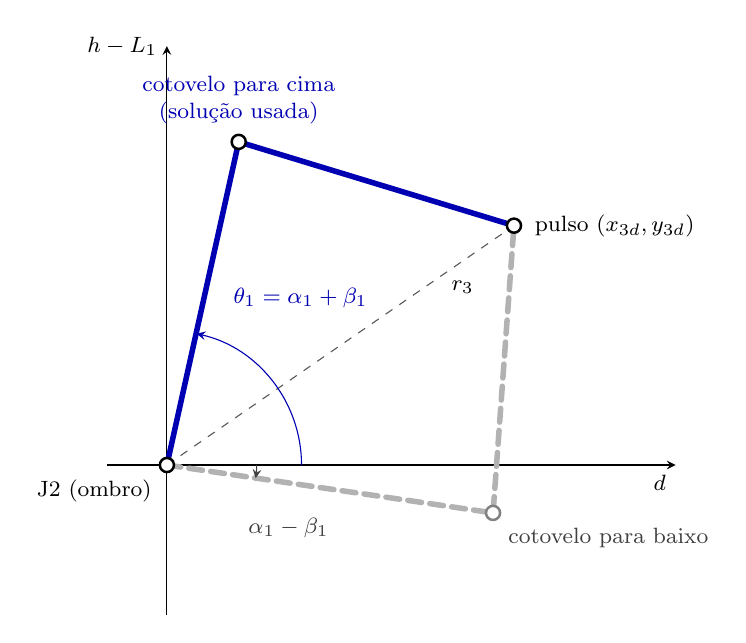
\begin{tikzpicture}[scale=0.38, >=stealth,
    elo/.style={line width=2pt, line cap=round},
    junta/.style={circle, draw, fill=white, line width=0.9pt, inner sep=1.8pt},
    cota/.style={gray!70!black, thin},
    ang/.style={->, thin},
    every node/.style={font=\footnotesize}]

  \draw[->, thin] (-2,0) -- (17,0) node[below left] {$d$};
  \draw[->, thin] (0,-5) -- (0,14) node[left] {$h - L_1$};
  \draw[cota, dashed] (0,0) -- node[pos=0.8, below right=-1pt, black] {$r_3$} (11.6,8.0);
  \draw[elo, gray!60, dash pattern=on 5pt off 3pt] (0,0) -- (10.9,-1.6) -- (11.6,8.0);
  \draw[elo, blue!70!black] (0,0) -- (2.4,10.8) -- (11.6,8.0);
  \node[junta] at (0,0) {}; \node[below left=2pt] at (0,0) {J2 (ombro)};
  \node[junta] at (2.4,10.8) {}; \node[above=3pt, blue!70!black, align=center] at (2.4,10.8) {cotovelo para cima\\(solução usada)};
  \node[junta, draw=gray] at (10.9,-1.6) {}; \node[below right=2pt, gray!50!black, align=center] at (10.9,-1.6) {cotovelo para baixo};
  \node[junta] at (11.6,8.0) {}; \node[right=4pt] at (11.6,8.0) {pulso $(x_{3d}, y_{3d})$};
  \draw[ang, blue!70!black] (4.5,0) arc[start angle=0, end angle=77.2, radius=4.5];
  \node[blue!70!black, anchor=west] at (1.9,5.6) {$\theta_1 = \alpha_1 + \beta_1$};
  \draw[ang, gray!50!black] (3,0) arc[start angle=0, end angle=-8.4, radius=3];
  \node[gray!50!black, anchor=west] at (2.4,-2.1) {$\alpha_1 - \beta_1$};
\end{tikzpicture}